% =====================================================================
%  CAPÍTULO 4 — ARQUITETURA DO SISTEMA
% =====================================================================

\chapter{ARQUITETURA DO SISTEMA}
\label{cap:arquitetura}

A arquitetura do \argus{} foi desenhada para garantir o máximo isolamento da
lógica de negócio em relação ao hardware e às interfaces visuais, assegurando
que o simulador funcione com alto desempenho tanto no computador quanto no
celular. Este capítulo descreve a \textit{stack} tecnológica, os princípios de
projeto adotados e a topologia de componentes do sistema.

\section{Visão geral e \textit{stack} tecnológico}
\label{sec:stack}

O \argus{} adota um modelo híbrido \textit{Desktop/Mobile} que centraliza a
lógica pesada em uma linguagem de sistema e reutiliza a interface web em
múltiplas plataformas. A \textit{stack} principal é composta por:

\begin{itemize}
    \item \textbf{Backend}: Go (Golang), escolhido pela eficiência no
        gerenciamento de concorrência (\textit{goroutines}) e pelo baixo
        consumo de memória, essenciais para manter conexões contínuas com
        múltiplos sensores BLE sem bloquear a \textit{thread} principal.
    \item \textbf{Bridge IPC}: o framework Wails \cite{wails2024}, que exporta
        os métodos Go para o \textit{frontend} por meio de \textit{bindings}
        assíncronos nativos.
    \item \textbf{Frontend}: JavaScript (ES6+) com Vite, focado em
        reatividade em tempo real (atualização de tela a 60~fps) e suporte
        nativo a temas claro/escuro.
    \item \textbf{Mobile}: Capacitor.js \cite{capacitor2024}, que encapsula a
        aplicação web em binários Android, reutilizando a interface e
        substituindo as chamadas de hardware de \textit{desktop} por APIs
        móveis.
    \item \textbf{Persistência}: SQLite \cite{sqlite2024} via ORM GORM
        \cite{gorm2024}, com repositórios granulares por entidade.
\end{itemize}

\section{Princípios de projeto: \textit{Clean Architecture}, \textit{Facade} e \textit{Repository}}
\label{sec:principios}

O sistema segue os princípios da \textit{Clean Architecture}
\cite{martin2017clean}, promovendo a separação estrita entre a camada de
apresentação, as regras de negócio e o acesso a hardware/rede. Essa organização
manifesta-se nas camadas:

\begin{enumerate}
    \item \textbf{Camada de apresentação (frontend em JavaScript)}: gerencia a
        interface de usuário, os gráficos Canvas e o barramento de eventos
        \code{TelemetryEventBus}, que atualiza a tela de forma assíncrona e
        desacoplada da chegada de dados.
    \item \textbf{Bridge IPC (Wails, \textit{desktop})}: camada de comunicação
        interprocesso que conecta a lógica do \textit{frontend} ao núcleo do
        \textit{backend}.
    \item \textbf{Camada de aplicação (controladores e casos de uso Go)}:
        estrutura a fachada \code{StorageFacade} e os controladores de treinos
        (\code{WorkoutController}) e de desafios (\code{ChallengeController}).
    \item \textbf{Camada de domínio e serviços \textit{core} (Go)}: compreende
        o motor físico de simulação baseado em dados GPX e o gerenciador de
        conexões Bluetooth LE (assinaturas GATT).
    \item \textbf{Camada de persistência (SQLite / FIT / serviços externos)}:
        mapeia os repositórios para o banco SQLite local e coordena a geração
        de arquivos \texttt{.FIT} e a transmissão segura às APIs do Strava e do
        Intervals.icu.
\end{enumerate}

\section{Topologia de componentes}
\label{sec:topologia}

A divisão lógica descrita na seção anterior é materializada nos pacotes do
projeto, localizados em \code{internal/}, organizados em \code{domain},
\code{usecase}, \code{service} e \code{repository}. Essa organização segue o
princípio da dependência dirigida ao domínio, no qual as entidades centrais
(definidas em \code{internal/domain}) não dependem de detalhes de
infraestrutura.

\section{Diagrama de componentes}
\label{sec:diagrama-arquitetura}

O diagrama da Figura~\ref{fig:arquitetura} ilustra a interação entre as camadas
do sistema, destacando a separação de responsabilidades e o fluxo de
comunicação entre o \textit{frontend} (JavaScript) e o \textit{backend} (Go).

\begin{figure}[htbp]
    \centering
    \caption{Arquitetura geral de componentes: \textit{Clean Architecture}}
    \label{fig:arquitetura}
    % =====================================================================
%  DIAGRAMA 1 — ARQUITETURA GERAL DE COMPONENTES
%  Fonte: autoria própria.
% =====================================================================
\begin{tikzpicture}[
    x=1cm, y=1cm,
    >=Stealth,
    box/.style={rectangle, draw, rounded corners=2pt, align=center,
      font=\footnotesize\sffamily, inner sep=4pt, minimum height=1.20cm,
      line width=0.6pt},
    layer/.style={font=\scriptsize\bfseries\sffamily, text=black!70, anchor=east},
    note/.style={font=\scriptsize\sffamily, text=black!65, align=center},
    arrow/.style={->, thick, draw=black!65},
]

    % -----------------------------------------------------------------
    % Apresentação compartilhada
    % -----------------------------------------------------------------
    \node[layer] at (-7.45, 9.10) {Apresentação};
    \node[box, fill=red!12, draw=red!60!black, minimum width=13.0cm,
          text width=12.6cm] (front) at (0.80, 9.10)
      {\textbf{Frontend JavaScript compartilhado (WebView)}\\
       HUD, mapa, gráficos, \texttt{TelemetryEventBus}, treino, desafio e resumo};

    % -----------------------------------------------------------------
    % Desktop: ponte, aplicação e domínio
    % -----------------------------------------------------------------
    \node[layer] at (-7.45, 7.15) {Ponte};
    \node[box, fill=purple!12, draw=purple!60!black, minimum width=9.0cm,
          text width=8.6cm] (wails) at (-1.20, 7.15)
      {\textbf{Desktop (Wails + Go)}\\
       Wails IPC: \textit{bindings} e eventos};

    \node[layer] at (-7.45, 5.50) {Aplicação};
    \node[box, fill=orange!14, draw=orange!65!black, minimum width=9.0cm,
          text width=8.6cm] (app) at (-1.20, 5.50)
      {\textbf{\texttt{app.go}}\\
       fachada, ciclo de sessão, recuperação e exportação};

    \node[layer] at (-7.45, 3.70) {Domínio};
    \node[box, fill=green!14, draw=green!45!black, minimum width=9.0cm,
          text width=8.6cm] (domain) at (-1.20, 3.70)
      {\textbf{Domínio e contratos}\\
       perfil, atividade, telemetria, \texttt{TrainerService},\\
       repositórios, GPX e FIT};

    % -----------------------------------------------------------------
    % Android: runtime separado
    % -----------------------------------------------------------------
    \node[box, fill=cyan!10, draw=cyan!55!black, minimum width=3.8cm,
          text width=3.4cm] (androidBridge) at (5.45, 7.15)
      {\textbf{Android (Capacitor)}\\
       WebView + plugin BLE\\
       física JavaScript};

    \node[box, fill=cyan!10, draw=cyan!55!black, minimum width=3.8cm,
          text width=3.4cm] (androidSession) at (5.45, 5.25)
      {\textbf{Sessão ao vivo}\\
       BLE, física JS e HUD};

    % -----------------------------------------------------------------
    % Adaptadores e infraestrutura
    % -----------------------------------------------------------------
    \node[layer] at (-7.45, 1.90) {Adaptadores};
    \node[box, fill=blue!12, draw=blue!55!black, minimum width=9.0cm,
          text width=8.6cm] (adapters) at (-1.20, 1.90)
      {\textbf{Adaptadores}\\
       BLE (FE-C/FTMS) · GPX · FIT/ZWO\\
       SQLite · IA/integrações};

    \node[box, fill=gray!15, draw=gray!60!black, minimum width=3.8cm,
          text width=3.4cm] (androidHardware) at (5.45, 3.35)
      {\textbf{Hardware BLE}\\
       rolo e sensores};

    \node[layer] at (-7.45, 0.10) {Infraestrutura};
    \node[box, fill=gray!15, draw=gray!60!black, minimum width=9.0cm,
          text width=8.6cm] (infra) at (-1.20, 0.10)
      {\textbf{Infraestrutura}\\
       rolo e sensores · arquivos · SQLite\\
       tiles · Strava/Intervals/Ollama};

    % -----------------------------------------------------------------
    % Conexões: verticais, sem cruzamentos
    % -----------------------------------------------------------------
    \draw[arrow] (front.south -| wails.north) -- (wails.north);
    \draw[arrow] (front.south -| androidBridge.north) -- (androidBridge.north);

    \draw[arrow] (wails.south) -- (app.north);
    \draw[arrow] (app.south) -- (domain.north);
    \draw[arrow] (domain.south) -- (adapters.north);
    \draw[arrow] (adapters.south) -- (infra.north);

    \draw[arrow] (androidBridge.south) -- (androidSession.north);
    \draw[arrow] (androidSession.south) -- (androidHardware.north);

    % Separação entre os runtimes; não é uma seta de chamada.
    \draw[dashed, draw=black!35] (3.45, -0.40) -- (3.45, 8.35);

    % Legenda
    \draw[arrow] (-6.60, -1.00) -- (-5.80, -1.00);
    \node[note, anchor=west] at (-5.70, -1.00) {chamada ou dependência};
    \draw[dashed, draw=black!35] (-1.55, -1.00) -- (-0.75, -1.00);
    \node[note, anchor=west] at (-0.65, -1.00) {fronteira de plataforma};

\end{tikzpicture}

\end{figure}

\section{Fluxo de telemetria em tempo real}
\label{sec:diagrama-telemetria}

A simulação de ciclismo virtual exige uma comunicação de baixíssima latência. O
diagrama de sequência da Figura~\ref{fig:telemetria} demonstra como os dados
trafegam do sensor até a renderização gráfica no momento do pedal, percorrendo
o serviço BLE em Go, o motor de simulação, a bridge Wails e o
\code{TelemetryEventBus} no \textit{frontend}.

\begin{figure}[htbp]
    \centering
    \caption{Fluxo sequencial de telemetria em tempo real}
    \label{fig:telemetria}
    % =====================================================================
%  DIAGRAMA 2 — FLUXO DE TELEMETRIA ENTRE SENSOR E INTERFACE
%  Fonte: autoria própria.
% =====================================================================
\begin{tikzpicture}[
    scale=0.85, every node/.style={transform shape},
    >=Stealth,
    actor/.style={rectangle, draw, rounded corners, minimum width=2.0cm,
      minimum height=0.7cm, align=center, font=\scriptsize\sffamily,
      fill=blueargus!15, text=blueargus!90!black, thick},
    edge node/.style={above, yshift=2pt, align=center, font=\tiny\sffamily},
    note/.style={font=\scriptsize\sffamily, align=center},
]

    % Lifelines
    \node[actor] (sensor) at (0,0) {Sensor BLE};
    \node[actor] (ble) at (2.6,0) {Serviço BLE\\Go};
    \node[actor] (sim) at (5.4,0) {Laço da\\sessão\\Go};
    \node[actor] (wails) at (8.2,0) {Wails IPC};
    \node[actor] (teb) at (10.8,0) {Telemetry\\EventBus\\JS};
    \node[actor] (canvas) at (13.4,0) {HUD /\\mapa};

    % Linhas tracejadas verticais
    \foreach \p in {sensor,ble,sim,wails,teb,canvas}
        \draw[dashed, black!40] (\p.south) -- (\p.south |- 0,-5.2);

    % Setas horizontais
    \draw[->, thick] (0,-1.4) -- node[edge node] {Notificação GATT}
        (2.6,-1.4);
    \draw[->, thick] (2.6,-2.2) -- node[edge node] {Telemetria}
        (5.4,-2.2);
    \draw[->, thick] (5.4,-3.0) -- node[edge node] {Amostra + estado}
        (8.2,-3.0);
    \draw[->, thick] (8.2,-3.8) -- node[edge node] {Evento}
        (10.8,-3.8);
    \draw[->, thick] (10.8,-4.6) -- node[edge node] {Publica}
        (13.4,-4.6);

    % Números sequenciais
    \node[note, font=\scriptsize\bfseries, above=3pt] at (sensor.north) {1};
    \node[note, font=\scriptsize\bfseries, above=3pt] at (ble.north) {2};
    \node[note, font=\scriptsize\bfseries, above=3pt] at (sim.north) {3};
    \node[note, font=\scriptsize\bfseries, above=3pt] at (wails.north) {4};
    \node[note, font=\scriptsize\bfseries, above=3pt] at (teb.north) {5};
    \node[note, font=\scriptsize\bfseries, above=3pt] at (canvas.north) {6};

    % Notas de comportamento
    \node[note, font=\tiny\itshape, text=black!60, anchor=north west,
        align=left, text width=12.4cm] at (-0.3,-5.35)
        {Chegada depende do sensor; não há taxa fixa.\\
         HUD recebe cada evento; o mapa limita a posição e anima a câmera.};

\end{tikzpicture}

\end{figure}

\section{Persistência e modelo de dados}
\label{sec:persistencia}

A persistência local é implementada sobre SQLite, acessado por meio do ORM
GORM \cite{gorm2024}. A aplicação mantém bancos de dados dedicados para o
histórico de atividades, os recordes de potência (curva MMP), o sistema de
gamificação e as classificações de eventos. As principais entidades do domínio
(\code{internal/domain}) são:

\begin{itemize}
    \item \code{UserProfile}: dados do atleta (nome, peso, FTP, frequências
        cardíacas, nível, XP, configurações e credenciais de integrações);
    \item \code{Activity}: sessão de treino concluída, com distância, elevação,
        métricas fisiológicas (NP, TSS, TRIMP, IF, desvio cardiovascular) e
        status de sincronização;
    \item \code{BikeComponent} e \code{ComponentReplacement}: componentes da
        bicicleta e seu histórico de substituições para o controle de desgaste;
    \item \code{EventRecord} e \code{SyncQueue}: classificações de eventos e a
        fila assíncrona de \textit{upload} para serviços externos;
    \item \code{AIConversation}: histórico de conversas do assistente de IA.
\end{itemize}

O acesso a essas entidades é orquestrado pela fachada
\code{StorageFacade}, que oferece uma interface limpa aos controladores Wails e
encapsula as transações entre os repositórios.

\section{Arquitetura móvel}
\label{sec:arquitetura-mobile}

No contexto móvel, o Capacitor encapsula a aplicação web e a comunicação com o
hardware é realizada pelo plugin \code{@capacitor-community/bluetooth-le}
\cite{capacitorble2024}, que expõe a antena BLE do dispositivo. Nessa
configuração, o motor de simulação física é executado em JavaScript
(\code{frontend/src/modules/CapacitorBluetoothService.js} e o motor portado),
permitindo o funcionamento autônomo do simulador em um smartphone sem o
\textit{backend} Go. A interface foi adaptada para operar em modo
\textit{landscape} (paisagem), priorizando a visibilidade do mapa 3D, como
ilustrado na Figura~\ref{fig:screenshot-mobile}.

\begin{figure}[htbp]
    \centering
    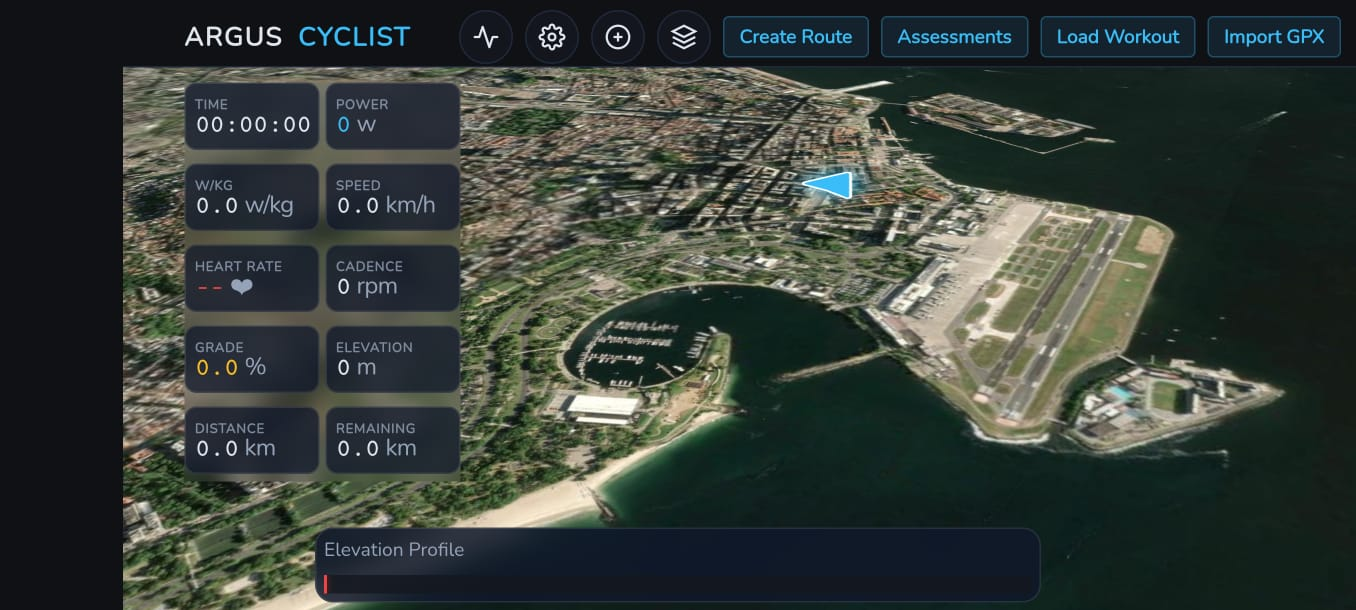
\includegraphics[width=0.85\textwidth]{figuras/screenshot-10-mobile}
    \caption{Aplicativo Android: HUD de simulação em modo \textit{landscape}}
    \label{fig:screenshot-mobile}
    \small Fonte: autoria própria.
\end{figure}

\section{Mapa mental do ecossistema}
\label{sec:diagrama-mapamental}

A Figura~\ref{fig:mapamental} apresenta o mapa mental do ecossistema \argus{},
organizando as principais funcionalidades e suas inter-relações.

\begin{figure}[htbp]
    \centering
    \caption{Mapa mental do ecossistema \argus{}}
    \label{fig:mapamental}
    % =====================================================================
%  DIAGRAMA 3 — MAPA MENTAL DO ECOSSISTEMA ARGUS CYCLIST
%  Fonte: autoria própria.
% =====================================================================
\begin{tikzpicture}[
    scale=0.7,
    transform shape,
    mindmap,
    every node/.style={concept, text=white, font=\sffamily\bfseries},
    root concept/.style={
      concept color=blueargus,
      minimum size=3.0cm,
      font=\large\bfseries,
      text width=2.8cm,
      align=center
    },
    level 1 concept/.append style={
      level distance=5.5cm,
      minimum size=2.7cm,
      font=\normalsize\bfseries,
      text width=2.0cm,
      align=center
    },
    level 2 concept/.append style={
      level distance=3.2cm,
      minimum size=2.2cm,
      font=\footnotesize\bfseries,
      text width=1.5cm,
      align=center
    },
]

      \node[root concept] {Argus\\Cyclist}
          % 1. Hardware BLE
          child[grow=0, concept color=greenargus!80!black] { node {Hardware\\BLE}
              child[grow=-35] { node {Heart\\Rate}}
              child[grow=0]   { node {Power\\Meter}}
              child[grow=35]  { node {FTMS\\Trainer}}
          }
          % 2. Simulação GPX
          child[grow=51.4, concept color=orangeargus] { node {Simulação\\GPX}
              child[grow=33.9] { node {Grade\\Dinâmica}}
              child[grow=68.9] { node {Elevação\\3D}}
          }
          % 3. Fisiologia
          child[grow=102.8, concept color=redargus!80!black] { node {Fisiologia}
              child[grow=67.8]  { node {NP / IF\\TSS}}
              child[grow=102.8] { node {PMC\\CTL/ATL}}
              child[grow=137.8] { node {Pw:HR}}
          }
          % 4. IA Coach Ollama
          child[grow=154.2, concept color=blueargus!60!white] { node {IA Coach\\Ollama}
              child[grow=136.7] { node {Planos\\ZWO}}
              child[grow=171.7] { node {Chat\\Local}}
          }
          % 5. Peças
          child[grow=205.7, concept color=greenargus] { node {Peças}
              child[grow=188.2] { node {Desgaste\\Linear}}
              child[grow=223.2] { node {Controle}}
          }
          % 6. Gamificação
          child[grow=257.1, concept color=orangeargus!70!black] { node {Gamificação}
              child[grow=239.6] { node {XP / Níveis}}
              child[grow=274.6] { node {Conquistas}}
          }
          % 7. Exportação
          child[grow=308.5, concept color=redargus] { node {Exportação}
              child[grow=291] { node {.FIT\\Garmin}}
              child[grow=326] { node {Strava\\API}}
          };
\end{tikzpicture}

\end{figure}
